\section{Method}
\label{sec:method}

\begin{figure*}[!t]
\centering
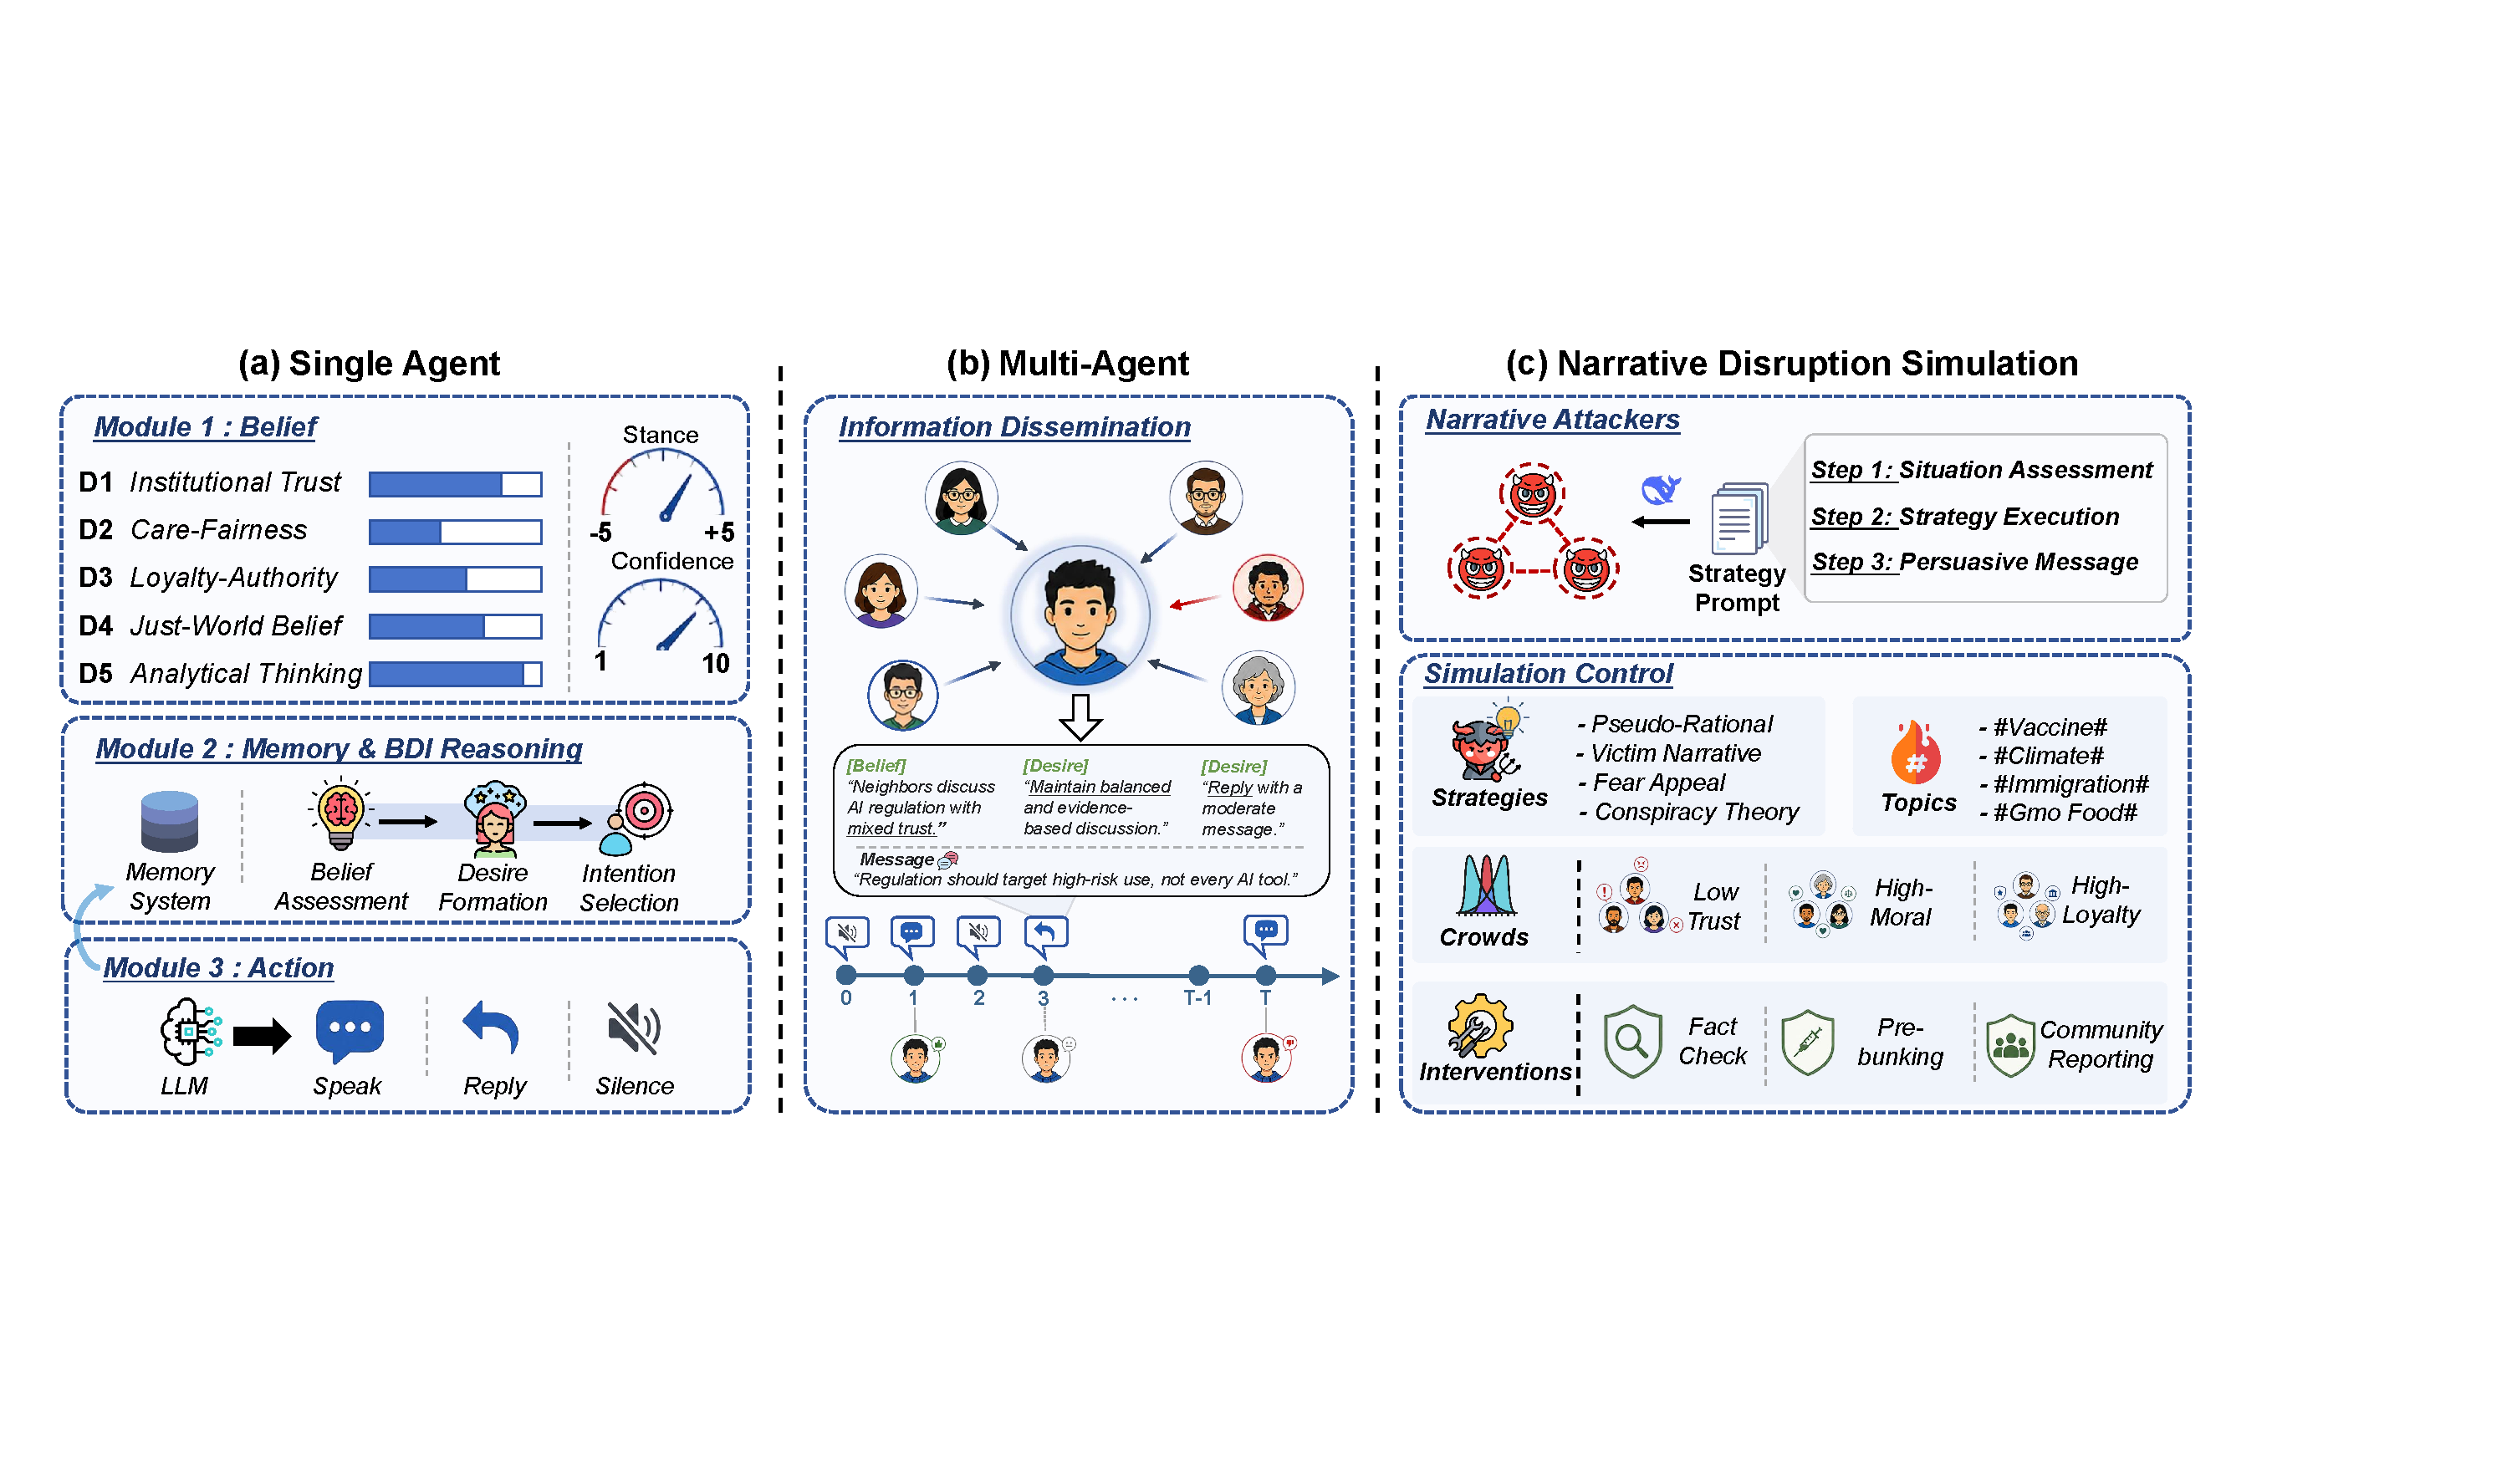
\includegraphics[width=\textwidth]{framework.pdf}
\caption{Overview of \textbf{NarrateSim}. (a)~A normal agent has a belief module (five static psychological dimensions plus dynamic stance and confidence), a memory and BDI reasoning module, and an action module that outputs communicative behaviour. (b)~Agents interact over a scale-free social network through synchronous rounds of local message exchange. (c)~The full simulation integrates normal agents, strategy-constrained narrative attackers, configurable interventions (pre-bunking, fact-checking, community reporting), and factorial experimental conditions across topics and population profiles.}
\label{fig:framework}
\end{figure*}

Our approach builds on advances in narrative framing analysis, computational manipulation detection, and LLM-based social simulation; a full discussion of related work appears in Appendix~\ref{sec:related}. We study this question with \textbf{NarrateSim}, a multi-agent simulation framework that places LLM-based agents in networked discussions on contentious topics. Figure~\ref{fig:framework} gives an overview. The rest of this section describes the agent architecture (\S\ref{sec:agent}), the multi-agent interaction mechanism (\S\ref{sec:interaction}), and the design of narrative attackers (\S\ref{sec:malicious}).

\subsection{Agent Architecture}
\label{sec:agent}

Each normal agent is modelled as a cognitive entity with three interconnected modules: a \emph{belief module} that encodes its psychological profile and current opinion, a \emph{memory and reasoning module} that supports structured BDI reasoning, and an \emph{action module} that maps reasoning outcomes into communicative behaviour.

\subsubsection{Belief Module}

Susceptibility to misinformation is not a single trait but arises from the interaction of multiple cognitive and personality factors~\citep{Ecker2022}. To capture this multidimensional nature, we equip each agent with a structured belief system consisting of static belief dimensions that define stable psychological dispositions, and dynamic belief states that evolve throughout the discussion.

\paragraph{Static Beliefs.}
Following the integrative framework of \citet{Ecker2022}, we operationalise five dimensions spanning cognitive style, worldview, and institutional orientation, each valued in $[1, 10]$:

\begin{itemize}
\setlength{\itemsep}{1pt}
\item $D_1$, \emph{Institutional Trust}: confidence in government, media, and experts~\citep{Mishler2001}.
\item $D_2$, \emph{Care--Fairness}: the individualizing moral foundation of empathy and harm prevention~\citep{Graham2013}.
\item $D_3$, \emph{Loyalty--Authority}: the binding moral foundation of group cohesion and social order~\citep{Graham2013, Feinberg2019}.
\item $D_4$, \emph{Just-World Belief}: tendency to view existing systems as fair~\citep{Lerner1980}.
\item $D_5$, \emph{Analytical Thinking}: disposition toward deliberative over intuitive reasoning~\citep{Pennycook2021}.
\end{itemize}

Each dimension is sampled from a configurable Gaussian distribution. The numeric vector $\mathbf{D}^{(i)}$ is then converted through a rule-based mapping into a natural-language personality description $\mathcal{P}^{(i)}$ that characterises the agent's attitudes in plain text. This description is embedded in the agent's system prompt and remains fixed throughout the simulation, enabling the LLM to reason with interpretable personality information.

\paragraph{Dynamic Beliefs.}
Each agent maintains two mutable states: a \emph{stance} $s_t^{(i)} \in \{-5, \ldots, +5\}$ indicating its position on the topic, and a \emph{confidence} $c_t^{(i)} \in \{1, \ldots, 10\}$ indicating commitment to that position. This two-dimensional representation follows opinion dynamics models that separate position from certainty~\citep{FriedkinJohnsen1990}. Initial values are sampled from configurable distributions and updated after every round through the BDI reasoning process.


\subsubsection{Memory and Reasoning Module}

\paragraph{Memory Mechanism.}
We use two complementary memory types for reasoning. \emph{Contextual perception} provides a snapshot of the current social environment: at each round the agent observes the most recent messages from its network neighbours. \emph{Experiential memory} is a sliding window $\mathcal{M}_t^{(i)}$ that stores the agent's own $K$ most recent round records ($K{=}10$), including past stances, actions, and messages. This allows the agent to track how its own views have evolved and maintain self-consistency.

\paragraph{BDI Reasoning.}
Before each contribution, the agent runs a structured reasoning step inspired by the BDI architecture~\citep{Bratman1987, Rao1995}. We treat this as a belief updating process where the agent revises what it currently thinks, decides what to say, and commits to how to say it. The three stages are:
\begin{itemize}
\setlength{\itemsep}{1pt}
\item \textbf{Belief}: updates the agent's view of the topic and surrounding sentiment from recent neighbour messages and its own past stances in experiential memory.
\item \textbf{Desire}: identifies what the agent feels compelled to express, including refraining when it has nothing new to add.
\item \textbf{Intention}: selects a concrete communicative action and produces a brief justification.
\end{itemize}
The reasoning output is formalised as:
\begin{equation}
\begin{aligned}
  \mathbf{O}_t^{(i)} &= \bigl(a_t^{(i)},\, \tau_t^{(i)},\, s_t^{(i)},\, c_t^{(i)},\, m_t^{(i)}\bigr) \\
  &= f_{\text{LLM}}\bigl(\mathcal{P}^{(i)},\, \mathcal{M}_t^{(i)},\, \mathcal{N}_t^{(i)},\, \mathcal{B}\bigr)
\end{aligned}
\label{eq:bdi_output}
\end{equation}
where $a_t^{(i)} \in \{\textsc{speak}, \textsc{reply}, \textsc{silent}\}$ is the action, $\tau_t^{(i)}$ is an optional reply target, $s_t^{(i)}$ and $c_t^{(i)}$ are updated stance and confidence, $m_t^{(i)}$ is the generated message, and $\mathcal{B}$ denotes behavioural constraints that regulate communicative norms to approximate authentic online discourse.


\subsubsection{Action Module}

The action module sits between the agent's internal reasoning and the social environment. It parses the structured LLM response to extract the chosen action, target, and message, and validates them against behavioural constraints so that the result stays consistent with online platform norms. A \textsc{speak} or \textsc{reply} broadcasts the generated message to neighbours and enters their contextual perception in the next round, while \textsc{silent} contributes no message but still updates the agent's internal state.


\subsection{Multi-Agent Interaction}
\label{sec:interaction}

Agents are connected through a Barab\'{a}si--Albert preferential-attachment network~\citep{Barabasi1999}, which produces a scale-free topology where a few highly connected hubs coexist with many low-degree nodes, approximating real online platforms. Network topology and random seeds are held constant across conditions to isolate the effects of manipulated variables. Each round, every agent observes recent messages from its immediate neighbours and produces a response via BDI reasoning (Eq.~\ref{eq:bdi_output}). This local visibility constraint causes opinions to spread gradually through the network.


\subsection{Narrative Attackers}
\label{sec:malicious}

We model narrative attackers as adaptive adversarial agents that represent coordinated influence operations~\citep{Ferrara2016}. Unlike template-based bots, our attackers observe the evolving discussion and generate contextually tailored persuasive messages each round.

\paragraph{Strategy-Constrained Generation.}
Each attacker is driven by a strategy prompt that specifies the persuasion mechanism to use and the tactics to avoid, preventing cross-strategy contamination so that observed effects remain attributable to the strategy itself. Before generating a message, the attacker assesses the recent discussion, identifies which participants seem most persuadable, and selects a concrete tactic for the round. It can reference specific participants, respond to emerging arguments, and adjust its language as the conversation develops.

\paragraph{Coordination and Evaluation.}
Each attacker has a broader view than any normal agent, seeing messages from across the network and a summary of the dominant sentiment. When several attackers act together, they post sequentially within a round and read what teammates have already said, taking complementary angles to diversify the attack surface. Narrative attackers carry no belief dimensions, do not update a stance, and are excluded from all metrics, so measured effects reflect the normal population alone. The specific strategies used appear in Section~\ref{sec:experiments}.
